\chapter[Studying karyopherins occupancy in the nuclear pore complex using biomimetic nanopores]{Studying karyopherins occupancy in the nuclear pore complex using biomimetic nanopores}
\chaptermark{Studying karyopherins occupancy using biomimetic nanopores}
\label{chapter_7}

\blfootnote{This chapter is based on a manuscript in preparation as: A. Fragasso, C.Dekker. Studying Karyopherins occupancy in the nuclear pore complex using biomimetic nanopores.}

%% The following annotation is customary for chapter which have already been
%% published as a paper.
%\blfootnote{ }

%% It is only necessary to list the authors if multiple people contributed
%% significantly to the chapter.
%\authors{Albert {\titleshape Einstein}}
%
%%% The '0pt' option ensures that no extra vertical space follows this epigraph,
%%% since there is another epigraph after it.
%\epigraph[0pt]{
%    Nature and nature's laws lay hid in the night; \\
%    God said `Let Newton be!' and all was light.
%}{Alexander Pope}
%
%\epigraph{
%    It did not last: the devil shouting `Ho. \\
%    Let Einstein be!' restore the status quo.
%}{Sir John Collings Squire}

\begin{abstract}
Nuclear Pore Complexes (NPCs) regulate all molecular transport between the nucleus and the cytoplasm in eukaryotic cells. Intrinsically disordered Phe-Gly nucleoporins (FG Nups) line the central conduit of NPCs and impart a selective barrier, where large proteins are excluded unless bound to a transport receptor (Karyopherin; Kap), which can freely pass the barrier. Two classes of models have been proposed to describe nuclear transport mechanistically, ‘FG-centric’, where FG Nups are the sole mediator of nuclear transport, and ‘Kap-centric’, where karyopherins participate in establishing the selective barrier. A consensus has not been reached yet. Here, we employ biomimetic nanopores, formed by tethering FG Nups to the inner wall of a solid-state nanopore, to show that a first population of Kaps are rapidly transported across the pore in $\sim$ms time, whereas a second population is stably assembled into the FG-mesh in the pore in a concentration-dependent manner. By analyzing the current noise fluctuations, we observe that such Kap binding induces an increase in rigidity of the FG-mesh as a function of concentration, a finding which we further corroborate with QCM-D experiments on FG Nup brushes. Our data show that Kaps do take part in forming the FG-barrier providing evidence for a ‘Kap-centric’ model of nuclear transport.
\end{abstract}
\newpage


\section{Introduction}
Molecular traffic between nucleus and cytoplasm is exclusively controlled by the Nuclear Pore Complex (NPC), a large protein complex (52 MDa in yeast\cite{Kim2018}) that forms a $\sim$40nm-diameter pore across the nuclear envelope that encloses the nucleus\cite{Veenhoff2007,Wente2000}. The NPC central channel is filled with a meshwork of intrinsically disordered FG-Nucleoporins (FG-Nups), that feature tandem phenylalanine-glycine (FG) amino acid sequences\cite{Terry2009,Yamada2010}. Strikingly, such a FG-mesh appears to behave as a selective gate\cite{Terry2009}: while molecules smaller than $\sim$40kDa ($\sim$5 nm in size) can pass through the pore unhindered, macromolecules with size >40kDa are blocked, unless they are bound to specific nuclear transport receptors (NTRs), such as karyopherins (Kaps), which can actively interact, partition, and translocate through the FG-Nup barrier. Major NTRs involved in nuclear import are Importin-$\beta$ in humans and Kap95 in yeast\cite{Stewart2007}.

In an effort to describe nuclear transport mechanistically, many models have been proposed\cite{David2014,Lim2015} which can be broadly categorized into two major classes: ‘FG-centric’ and ‘Kap-centric’ models. The first class of FG-centric models, which include the ‘virtual-gate’\cite{Rout2003}, ‘selective-phase’\cite{Frey2006,Frey2007}, and ‘forest’\cite{Yamada2010} models, regard the FG-Nup barrier as the sole important ingredient to achieve selective transport. In such scenario, Kaps act as mere transporters, \emph{i.e.} they do not take part in establishing the selective barrier.

By contrast, Kap-centric models\cite{Kapinos2014}, such as the ‘reduction of dimensionality’\cite{Peters2005}, ‘reversible collapse’\cite{Lim2007}, and ‘molecular velcro’\cite{Schleicher2014} models, predict that a part of the population of Kaps (‘slow-phase’) acts an integral, resident component of the NPC\cite{Kapinos2014,Kapinos2017}, while a second population of Kaps consists of transporters (‘fast-phase’). According to this idea\cite{Lim2015}, Kaps that feature binding affinities (K\textsubscript{D}) to the FG-mesh <1 $\mu$M, would bind strongly and occupy most of the available FG-repeats as a result of multivalent interactions, hence forming the slow-phase population. Notably, each Kap can bind multiple FG-repeats (up to $\sim$10 FG-binding sites in Kap$\beta$1\cite{Bayliss2000}), while at the same time a single FG-Nup can bind multiple Kaps, thus giving rise to a complex multivalent-binding condensate. Saturation of available FG-repeats by the slow-phase Kaps would then result in a lowered affinity between the Kap-laden FG-mesh and additional free Kaps (fast-phase) down to K\textsubscript{D}>10$\mu$M. Importantly, such a decreased affinity would explain the exceptionally fast transit times of Kaps ($\sim$5 ms) observed in vivo\cite{Dange2008}.


While experimental evidence has been provided in support of both classes of models, a general consensus has not yet been achieved. The difficulty in settling the debate stems from the complexity of the NPC in its physiological state, featuring a central mesh of $\sim$200 unstructured FG-Nups that are confined into a $\sim$40nm pore that is constantly being crossed by NTR-cargo molecules ($\sim$1000 molecules per second) in both directions, combined with the limited spatiotemporal resolution of current imaging techniques\cite{Kim2018,Veenhoff2007,Ribbeck2001}.


To probe nuclear transport through the FG-mesh, artificial mimics of the NPC have been successfully reconstituted that recapitulate the selective binding and transport behavior observed \emph{in vivo}\cite{Jovanovic-Talisman2009,Kowalczyk2011a,Eisele2010a,Malekian2018,Schoch2012,Schmidt2015}. Prominent examples are the biomimetic nanopores, where $\sim$30-50 nm solid-state nanopores are chemically functionalized using a single type of FG-Nup (\emph{e.g}. Nsp1 or Nup98) and translocations of Kaps through the reconstituted FG-mesh are monitored in real-time optically\cite{Jovanovic-Talisman2009} or electrically\cite{Kowalczyk2011a,Ananth2018,Fragasso2021}. Although much knowledge has been gained in terms of a physical understanding of the FG-mesh and its ability to impart a selective barrier, a direct assessment is still lacking of the properties of such pore-confined FG-mesh as a function of Kap concentration in light of the various transport models.


Here, we employ biomimetic nanopores to obtain experimental evidence on the interaction between Kaps and Nsp1 in nanopores, in an attempt to discriminate between the two major theories of transport. Building on previous work from Ananth \emph{et al.}\cite{Ananth2018}, which established that Nsp1-coated pores behave selectively, \emph{i.e.} allowing Kap95 through while blocking other inert molecules of similar size, we investigate here the behavior of Nsp1-coated pores against increasing concentrations of Kaps.


Our data are found to support a Kap-centric model. Measurements of the ionic current through the biomimetic nanopores show that fast translocations of Kaps are observed, consistent with previous findings\cite{Ananth2018}, but on top of that, a population of Kaps is found that resides permanently in the pore, and this population grows as a function of Kap concentration. By studying the noise spectra of the current traces, we observe a gradual decrease in 1/f noise as more Kaps are incorporated into the pore, consistent with a decrease in the collective fluctuations of the FG-Nups and an increase in the rigidity of the Nsp1 mesh. We complement our nanopore data with QCM-D affinity experiments that show a similar concentration-dependent occupancy of Kap95 into Nsp1 brushes as well as an increase in layer rigidity. By thus showing that a population of Kaps is stably bound to the Nsp1 mesh in a biomimetic nanopore at any given concentration, these data support the idea that Kaps do take part in establishing the NPC barrier, which should be accounted for in any mechanistic modeling of nuclear transport.


\section{Results}
\subsection{Electrical transport through Nsp1-coated pores shows an increase in Kap95 occupancy as a function of Kap95 concentration}
To perform ion current measurements through Nsp1-coated pores (Fig.\ref{fig:fig7.1.1}a), solid-state nanopores were fabricated onto glass-supported freestanding 20nm-thick SiN\textsubscript{x} membranes using a transmission electron microscope (TEM, see ‘Methods’ section). Chips were mounted in a custom-built Teflon flow-cell system to allow for quick exchange of bulk solution from the two opposite compartments surrounding the chip. Conductance measurements were initially performed on freshly drilled nanopores, which, as expected, exhibited fully ohmic behavior, \emph{i.e.} linear current-voltage (I-V) characteristics. Figure \ref{fig:fig7.1.1}a shows the I-V plot of a bare 55 nm pore. Subsequently, pores were functionalized with Nsp1 using a 3-step self-assembled-monolayer chemistry (SAM) as described in previous work\cite{Fragasso2021} (see ‘Methods’), which yielded a $\sim$50\% decrease in conductance (Fig.\ref{fig:fig7.1.1}b). 

Next, Kap95 was flushed on the \emph{cis}-chamber which resulted in a further decrease of the pore conductance. This in itself directly provides a first sign that Kap95 was incorporated within the pore volume. Figure \ref{fig:fig7.1.1}c (bottom) compares the three (I,V) characteristics of a bare pore (black), Nsp1-coated (red), and Nsp1-coated pore with 1.9 $\mu$M of Kap95 present in bulk solution (green), where the latter shows a further $\sim$50\% decrease in conductance compared to the Nsp1-coated pore, indicating the presence of Kap95 molecules in the pore.


To assess the pore-occupancy of Kap95 as a function of concentration, we titrated Kap95 from about 100-2000 nM (Figure \ref{fig:fig7.1.2}a), finding the pore conductance to decrease monotonously in a step-wise manner as higher concentrations of Kaps were flushed into the \emph{cis}-chamber, which clearly indicates that additional Kaps are being incorporated into the Nsp1-mesh for increasing Kap95 concentration. Interestingly, we found that transient dips in the current, corresponding to fast Kap95 translocation events, were simultaneously present as well on top of the decreased current baseline, which occurred only when the bulk concentration was $\sim$100nM, in line with previous measurements\cite{Ananth2018}. We attribute the absence of current spikes at higher Kap95 concentrations to excessive pore crowding which negatively affects the SNR in such current-based detection system.

\begin{figure}[!htbp]
	\centering
	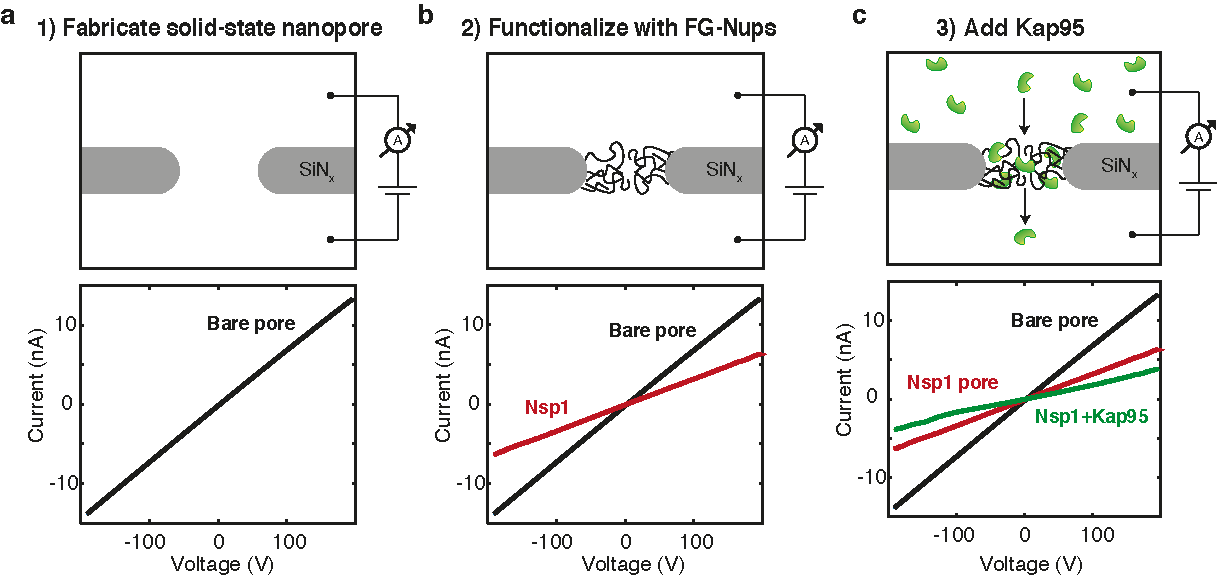
\includegraphics[width=1\linewidth]{figures/Figure7.1.1.pdf}
	\caption{Current measurements of Nsp1-coated pores as a function of Kap95 concentration. a,  Top: schematic showing the bare pore measurement system. Bottom: (I,V) characteristics of a bare 55 nm pore. b-c,  Same as (a) but for a Nsp1-coated pore without (b) and with (c) 1.9$\mu$M Kap95 present in the \emph{cis}-chamber (top part).}
	\label{fig:fig7.1.1}
\end{figure}

As a control, we repeated the same experiment by injecting increasing concentrations of BSA (Bovine Serum Albumine) in the \emph{cis}-chamber from $\sim$2-20 $\mu$M (Figure \ref{fig:fig7.1.2}c). Here we found that, unlike for Kap95, no significant change in the current baseline was observed. Importantly, this indicates that the interaction observed between Kap95 and Nsp1 is a result of specific protein-protein interactions, and not merely due to, \emph{e.g.}, electrostatic pulling of the protein into the Nsp1-mesh. Repeating the experiment on different pore sizes resulted in a similar decreasing trend of the pore conductance as a function of Kap95 concentration (Fig.\ref{fig:fig7.1.2}d). 


\begin{figure}[!htbp]
	\centering
	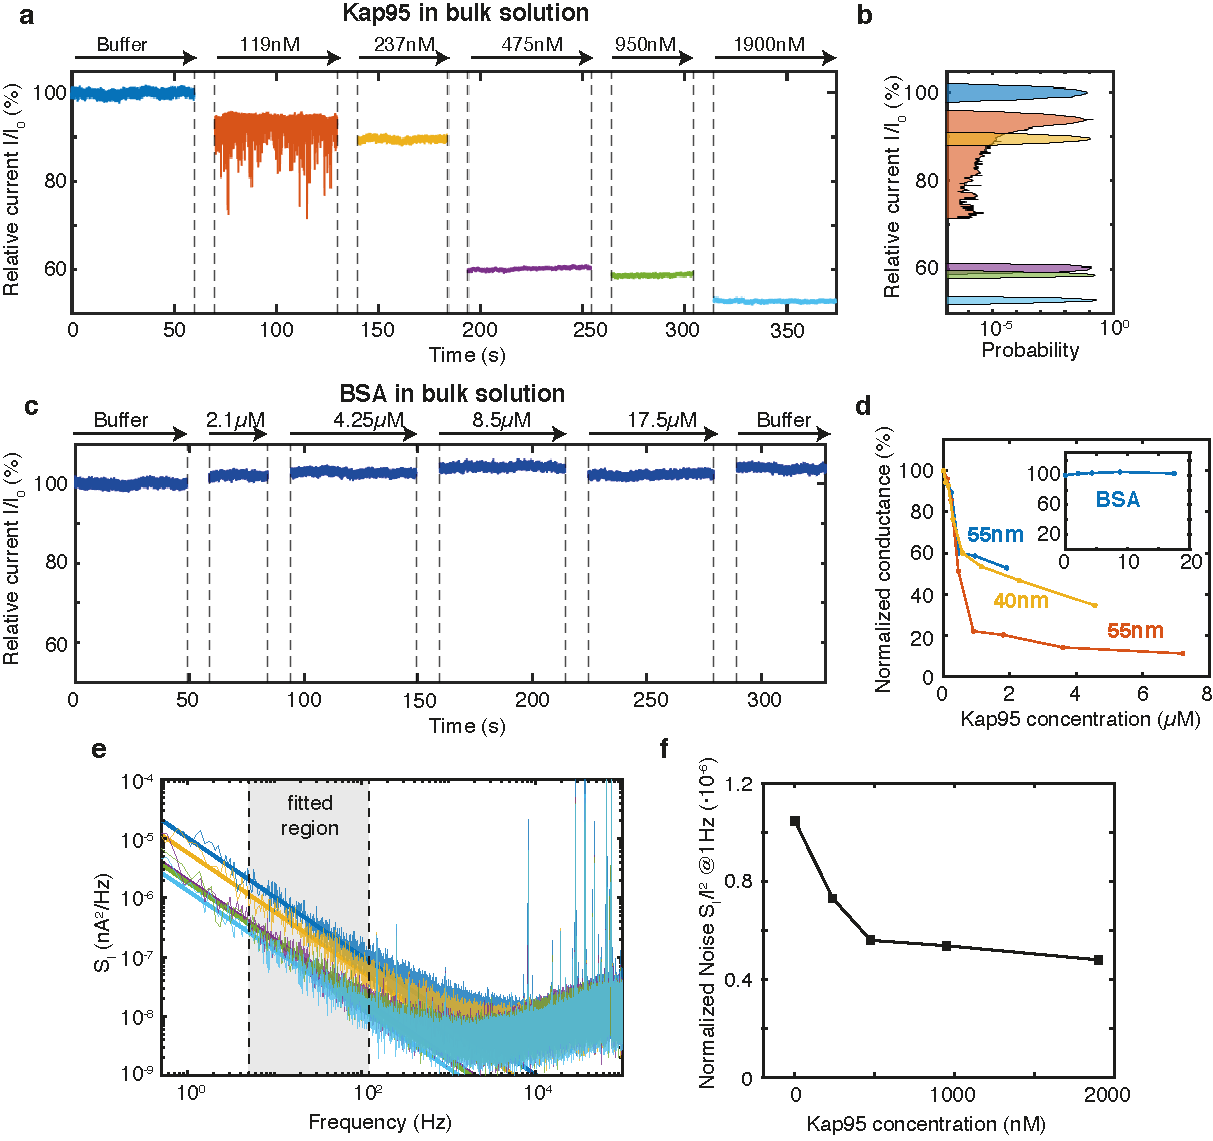
\includegraphics[width=1\linewidth]{figures/Figure7.1.2.pdf}
	\caption{a, Concatenated current traces representing a Kap95 titration from 119-1900nM, revealing a decrease of the nanopore current up to almost $\sim$50\% of the initial value. b, Histogram of the current traces illustrated in (a). c, Concatenated current traces representing a BSA titration from 2-20$\mu$M, showing no sign of current decrease. d, Normalized conductance for different nanopores vs Kap95 concentration. Inset: normalized conductance for a 55 nm pore vs BSA concentration (same units as in d applies). e, PSD spectra of the current traces shown in (a), same color coding as in (a) applies. f, Normalized noise $A=S_I (1Hz)/I^2$, as a function of Kap95 concentration. Fit to the noise data for 119 nM concentration was excluded due to the presence of a pronounced Lorentzian component originating from the Kap95 translocations (see Refs.\cite{Fragasso2020,Machlup1954}) which yielded a poor fit of Hooge’s model to the data.}
	\label{fig:fig7.1.2}
\end{figure}


Next, we analyzed the power spectral density (PSD) of the ionic current as a function of Kap95 concentration, \emph{i.e.} the frequency spectrum of the power of the current signal. For biomimetic nanopores, the increase in low-frequency (1-100 Hz) 1/f noise upon addition of the Nups has been typically associated to spatiotemporal fluctuations of FG-Nup proteins in the pore channel\cite{Kowalczyk2011a,Ananth2018,Fragasso2021}.  Indeed we also report an increase in 1/f noise when comparing the bare vs Nsp1-coated pore (Fig.\ref{fig:fig7.5}). More interestingly, we furthermore observe an overall decreasing trend in the 1/f noise as a function of Kap concentration (Fig.\ref{fig:fig7.1.2}e,f). To properly compare the magnitude of 1/f noise for different current traces, we fitted the low-frequency region (5-100 Hz) of the PSD (grey area in Fig.\ref{fig:fig7.1.2}e) using Hooge’s model\cite{Hooge1976}, which is commonly used to describe 1/f noise in solid-state nanopores\cite{Smeets2009,Smeets2008,Fragasso2019,Fragasso2020}, where the current PSD ($S_I$) is expressed as  $S_I=\alpha_H I^2/N_c f=AI^2/f$ , where,  $\alpha_H$ is the Hooge parameter that quantifies the strength of the 1/f noise, $I$ is the through-pore current, $N_c$ is the number of charge carriers within the pore volume which depends on salt concentration and pore geometry, $f$ is the frequency, and $A=\alpha_H/N_c=S_I (1Hz)/I^2$ is the fit parameter, which is a measure of the noise magnitude normalized by the square of the current. Figure \ref{fig:fig7.1.2}f shows a clear decreasing trend for $A$ as a function of Kap95 concentration, indicating that a higher Kap occupancy resulted in a decrease of the 1/f noise. This is suggestive of an increase in overall rigidity of the Nsp1-mesh in the pore. This finding is in line with the observed increase in rigidity of Nsp1 brushes grafted on a planar geometry upon Kap95 binding as reported in our QCM-D measurements (see below), as well as in previous works\cite{Eisele2010a,Wagner2015}.


\subsection{Analysis of fast Kap95 translocations through an Nsp1 pore }
We then characterized the translocation events of Kap95 (fast phase) when increasing the applied voltage from 50 to 200mV. For each event, we measured the current blockade, which to a first approximation is proportional to the volume of the translocating molecule, and dwell time, which corresponds to the time the translocating protein spends in the pore which depends on the specific protein-pore interactions. In Figure \ref{fig:fig7.2}a we show examples of current traces where each current spike correspond to a single Kap95 translocation event. Figure \ref{fig:fig7.2}b illustrates some characteristic translocation events at different voltages in higher resolution.

\begin{figure}[!htbp]
	\centering
	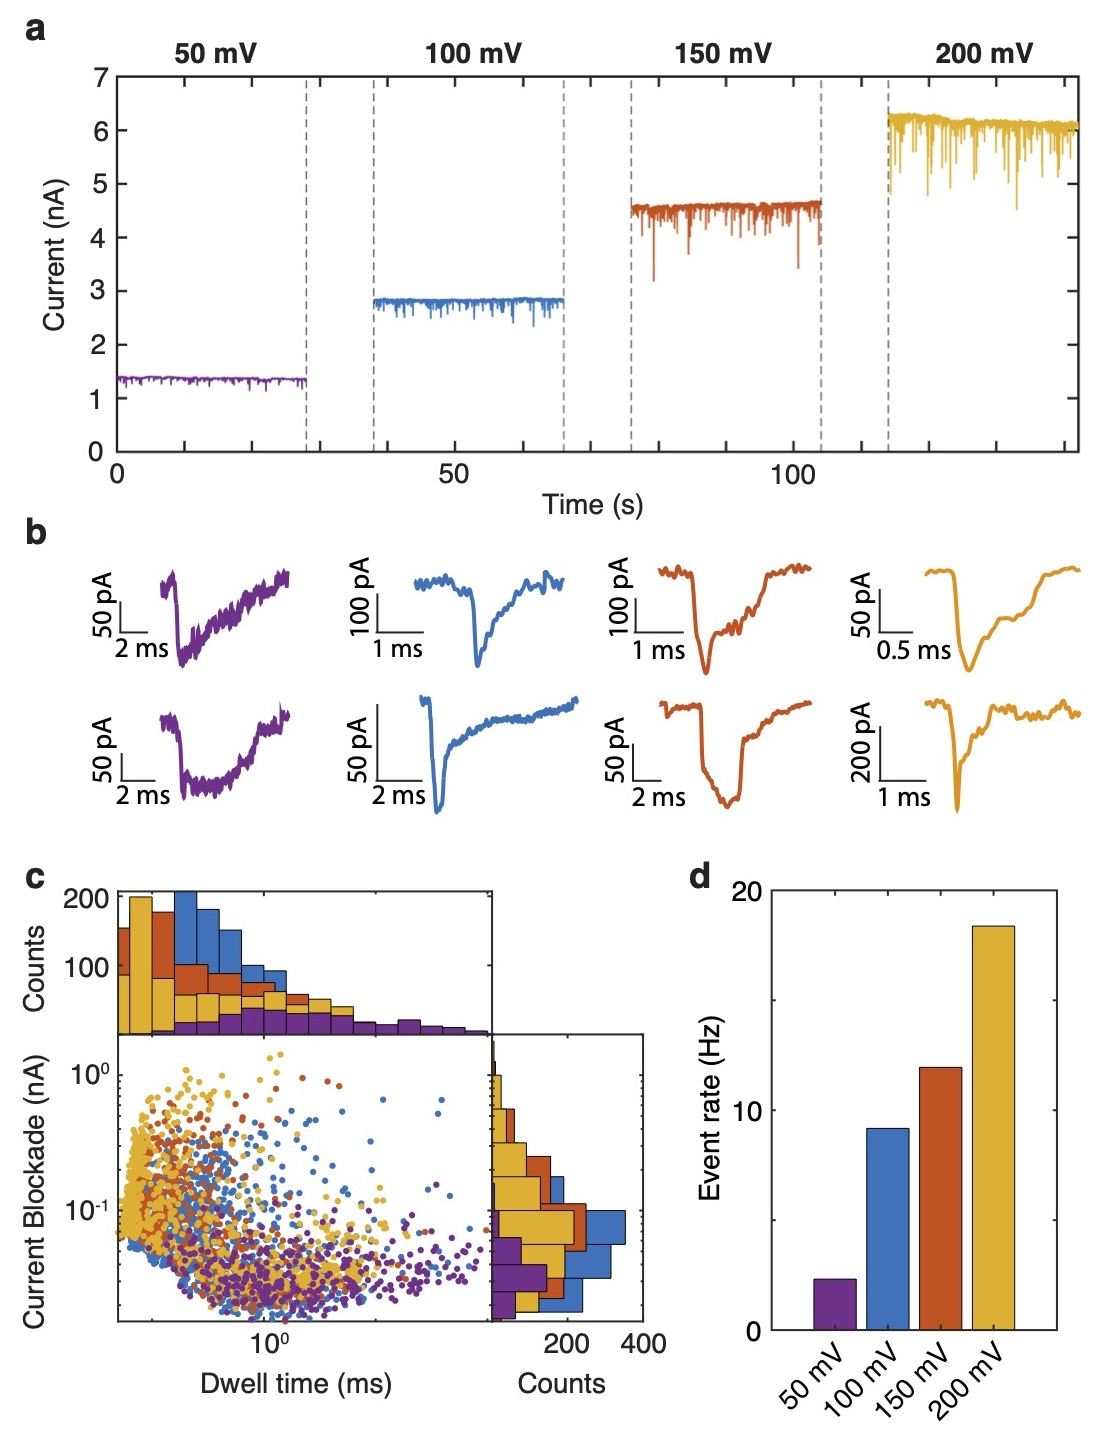
\includegraphics[width=1\linewidth]{figures/Figure7.2}
	\caption{Event analysis of Kap95 translocations. a, Current traces showing single-molecule translocations of Kap95 through a Nsp1-coated pore under 50mV (purple), 100mV (blue), 150mV (red), 200mV (yellow). Additional examples are shown in Figure \ref{fig:fig7.6}. b, Characteristic Kap95 translocation events at different voltages. c, Scatter plot of the current blockade vs dwell time of the translocation events for different voltages. Histograms for both dwell time and current blockade are logarithmically binned. d, Event rate of the translocations, defined as number of events per second, for increasing applied voltage. Color coding of b-d are the same as for a.}
	\label{fig:fig7.2}
\end{figure}

As expected, conductance blockades at different voltages are found to be comparable: 76$\pm$2 nS at 50mV (N=310, errors are S.E.M.), 80$\pm$2 nS at 100mV (N=1206), 77$\pm$3 nS at 150mV (N=687), and (64$\pm$3 nS) at 200mV (N=820). By contrast, for values of the applied bias >50mV we observed a drastic decrease of the resident time of the protein being in the pore due to a stronger electrophoretic force driving the protein, which goes from 7.8$\pm$0.8ms for 50mV (N=310, errors are S.E.M.) to about $\sim$1ms at higher voltages: 1.2$\pm$0.1ms for 100mV (N=1206), 0.8$\pm$0.2ms for 150mV (N=687), and 1.1$\pm$0.1ms for 200mV (N=820). Notably, the translocation events that are the least affected by the applied bias, namely acquired under 50mV, result in dwell times of $\sim$8ms that are remarkably close to the $\sim$5ms observed in vivo. Additional examples of current traces are show in Fig.\ref{fig:fig7.6}.

Lastly, the event rate of translocations, calculated as number of translocation events per second, was observed to increase as a function of applied voltage by almost an order of magnitude when increasing the bias from 50mV to 200mV (Fig.\ref{fig:fig7.2}d). This is indicative of an increase in the capture radius as a function of voltage\cite{Otto2013}, defined as the radius of the hemisphere surrounding the pore wherein the electrostatic force driving the protein to the pore overtakes simple diffusion.


\subsection{Kap95 occupancy in a Nsp1 brush increases with Kap95 concentration}
To assess the binding of Kap95 to Nsp1 brushes, we complemented our nanopore data with measurements using a quartz-crystal-microbalance with dissipation monitoring (QCM-D). For this, we monitored the resonance frequency shift ($\Delta$f) of the crystal, which is proportional to amount of adsorbed mass, and the dissipation shift ($\Delta$D), which depends on the viscoelastic properties of the adsorbed layer.

\begin{figure}[!htbp]
	\centering
	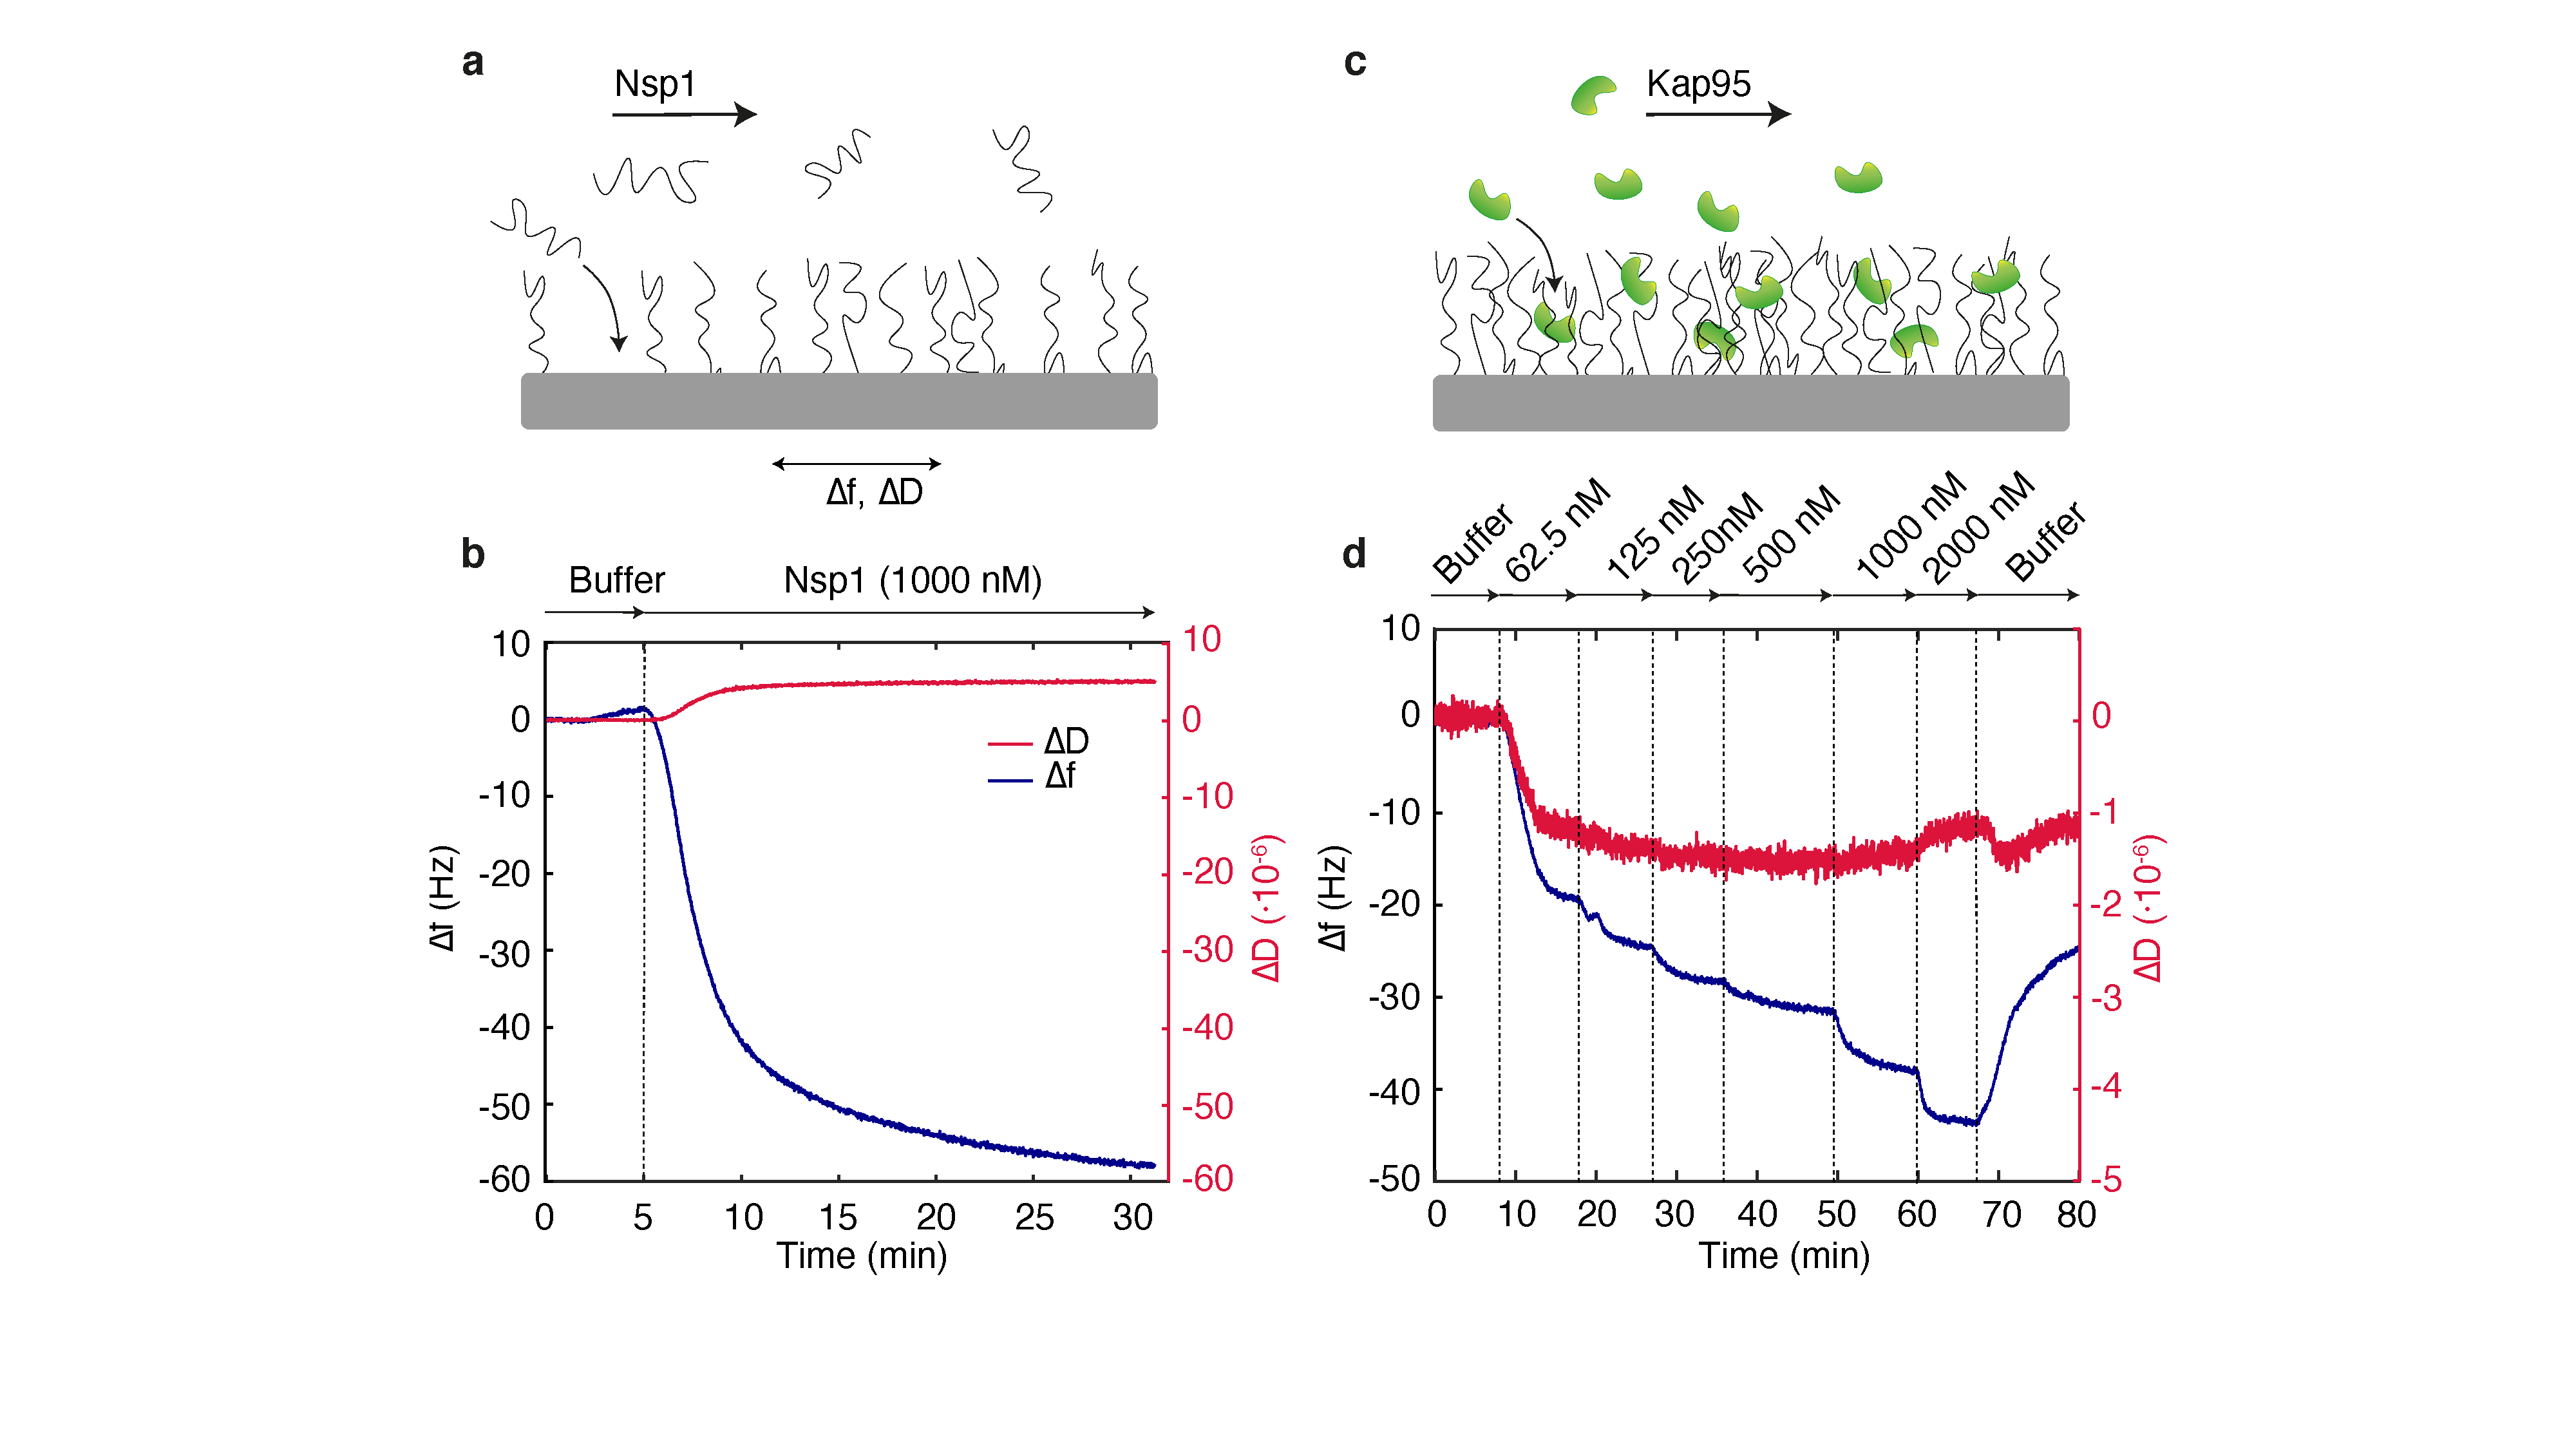
\includegraphics[width=1\linewidth]{figures/Figure7.3.pdf}
	\caption{Probing Kap95 binding to Nsp1 with QCM-D. a,c,  Schematics showing Nsp1 coating (a) and Kap95 injection (b) onto the quartz chip. b, Recordings of frequency (blue) and dissipation (red) shifts vs time when injecting 1000 nM Nsp1 onto the gold-coated chip surface. Binding of the molecule is revealed by the negative shift in resonance frequency, whereas the increase in dissipation is consistent with the formation of a hydrated Nsp1 brush. d, Frequency and dissipation shifts vs time upon Kap95 injection onto a Nsp1-coated surface at increasing concentrations from 62.5-2000 nM.}
	\label{fig:fig7.3}
\end{figure}

\noindent After a cleaning routine (see Methods), gold-coated chips were first functionalized with Nsp1 (Fig.\ref{fig:fig7.3}a,b) which features a cysteine on its C-terminus that is used for conjugation to the gold surface. Incubation of the Nsp1 protein with the gold surface resulted in a $\Delta$f$\sim-58$Hz, indicating the formation of a dense Nsp1-brush (cf. Ref.\cite{Eisele2018}). Subsequently we passivated the remaining gold exposed in between Nsp1 molecules using 1-mercapto-11-undecylte-tri(ethyleneglycol) (MUTEG) (see details in Ref.\cite{Fragasso2021}).

Kap95 was flushed in at increasing concentrations in the range (62.5-2000 nM), which resulted in a step-wise decrease in frequency shift – indicating a concentration-dependent Kap95 adsorption onto the Nsp1-brush (Fig.\ref{fig:fig7.3}c,d). This observation is perfectly in line with previous reports\cite{Eisele2010a,Wagner2015}, as well as our nanopore data where we report a concentration-dependent incorporation of Kap95 into the Nsp1 pore mesh. 


Additionally, we observed a striking decrease in dissipation $\Delta$D $\sim$ $-1\times10^{-6}$ as soon as the lowest Kap95 concentration (62.5 nM) was injected, which indicates an increase of the layer rigidity\cite{Eisele2010a,Reviakine2011,Eisele2013}. This finding is in line with the notion of ‘collapse’ of the Nsp1 brush, consistent with a decrease in brush height upon Kap binding, reported by Wagner \emph{et al.}\cite{Wagner2015}, where the interaction between Nsp1 and Kap$\beta$1 was monitored optically by surface-plasmonic-resonance (SPR). Importantly, such an increase in layer rigidity measured by QCM-D is consistent with the decrease in 1/f noise observed in our nanopore experiments.


\subsection{Support for the Kap-centric model of nuclear transport}
It is of interest to discuss these data in the context of the various models for nuclear transport. Most importantly, our nanopore data show that while a population of fast Kaps are rapidly translocating through the pore in a timescale of milliseconds, a second population of quasi-permanent Kaps is also present (Fig.\ref{fig:fig7.4}a) which appears in the ion current data as a stable, concentration-dependent, decrease of the current baseline. Moreover, binding of Kap95 appears to have a ‘stiffening’ effect on the Nsp1-mesh, as observed by the overall decrease of the 1/f noise in the nanopore and the dissipation in QCM-D.

\begin{figure}[!htbp]
	\centering
	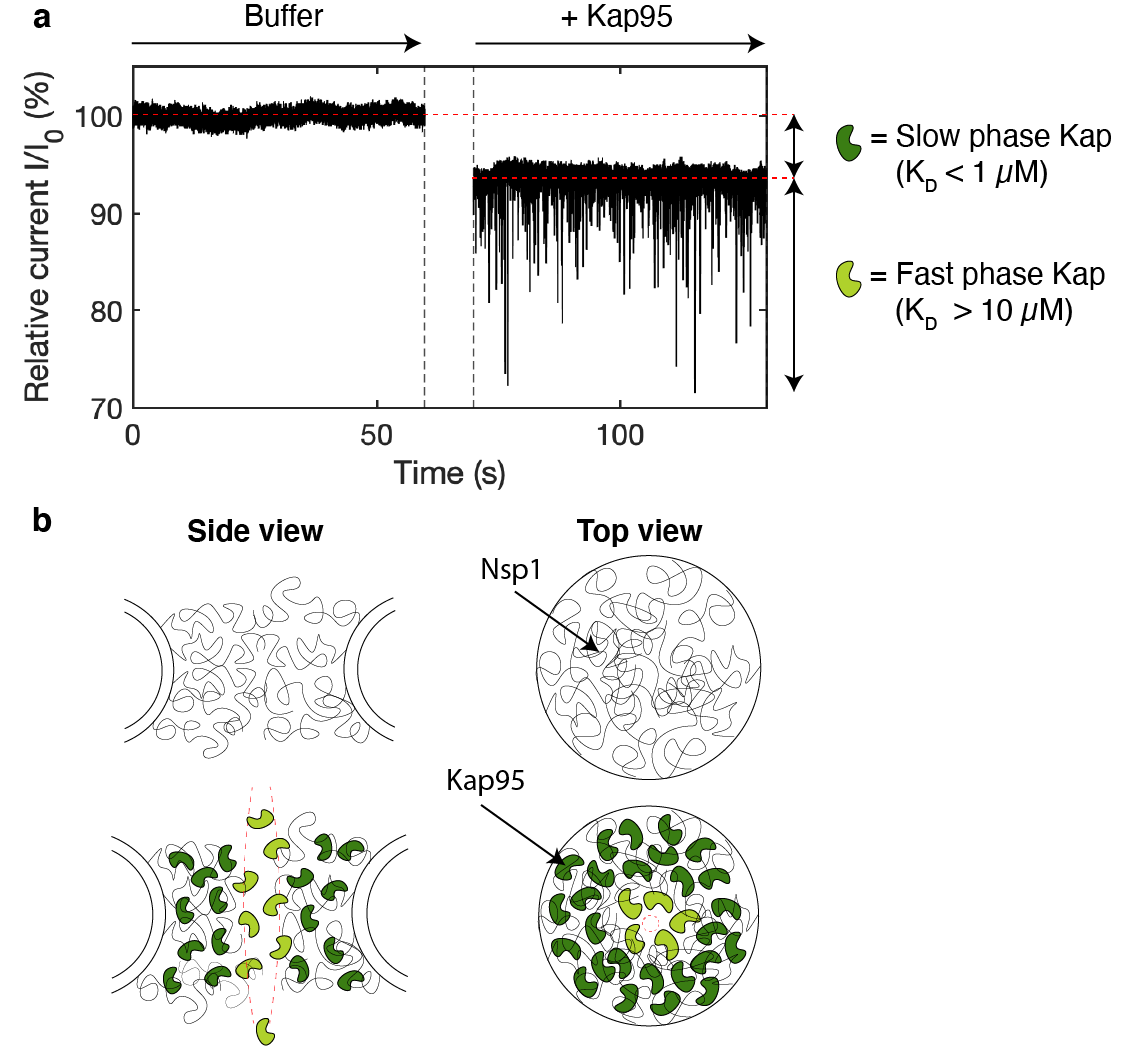
\includegraphics[width=1\linewidth]{figures/Figure7.4.png}
	\caption{Kap-centric transport model. a, Nanopore current traces showing baseline decrease, associated with ‘slow-phase’ Kaps biding stably to Nsp1, as well as transient spikes, which indicate ‘fast-phase’ ($\sim$ms) Kap95 translocations through the pore. b, Schematics of the coated pore side (left) and top (right) views in the absence (top) and presence (bottom) of Kaps, picturing the Kap-centric model (as in Kapinos et al.\cite{Kapinos2014}). ‘Slow-phase’ Kaps (dark green) reside towards the pore rim and cause the opening of a central channel where ‘fast-phase’ Kaps (light green) are allowed to rapidly translocate by weakly interacting with the saturated FG-mesh.}
	\label{fig:fig7.4}
\end{figure}

A possible arrangement of the two Kap95 populations (fast vs slow) within the nanopore was suggested by Kapinos \emph{et al.} 2014\cite{Kapinos2014} and illustrated in Figure \ref{fig:fig7.4}b. Here, slow Kaps that bind the Nsp1 mesh with high avidity (<1$\mu$M) would induce a collapse of the Nsp1-mesh towards the pore rim, resulting in the opening of a central channel (Fig. \ref{fig:fig7.4}b, red dashed lines), through which fast Kaps can rapidly diffuse through in $\sim$ms time. This is in line with our data showing a stable drop of the baseline due to slow Kaps binding to the FG-mesh while increasing its stiffness (Fig.\ref{fig:fig7.1.2}a,f), which may be associated with the formation of a central opening for the fast-diffusing Kaps resulting in the observed fast ($\sim$7.8 ms at 50mV, Fig.\ref{fig:fig7.3}) translocation events. Our data are also compatible with the ‘reduction-of-dimensionality’\cite{Peters2005} and ‘molecular velcro’\cite{Schleicher2014} models, where translocating Kaps would cross the pore following a 2D-random walk on the collapsed, Kap-saturated layer of FG-Nups. Formation of a channel opening upon Kap binding is also consistent with in vivo super-resolution data from Ma \emph{et al.}\cite{Ma2012}, where increasing the concentration of Imp$\beta$ from 1 nM to 15 $\mu$M in human cells resulted in higher NPC permeability to large 70 kDa Dextran molecules. 


\section{Conclusion}
In this work, we investigated the interaction between the yeast transporter Kap95 and FG-nucleoporin Nsp1 using biomimetic nanopores. We identified two distinct Kap95 populations: slow Kaps that bind stably to the Nsp1 mesh causing a permanent decrease in the current baseline, and fast Kaps that rapidly translocate the pore on a $\sim$ms timescale. The population of slow Kaps was found to increase in a concentration-dependent manner as revealed by the step-wise decrease of the pore conductance. The net decrease in 1/f noise in the current signal, together with the decrease in dissipation measured by QCM-D, for increasing Kap95 concentrations points to an increased rigidity of the Nsp1-mesh for increased Kap occupancy. 

Taken together, our data are in agreement with the Kap-centric model for nuclear transport. It opens the way to further studies using more physiological scenarios by, \emph{e.g}., introducing the Kap95 binding partner, Kap60, and studying RanGTP-assisted dissociation when this is added on the \emph{trans}-side of the pore. Other platforms that avoid the use of an applied voltage could also be envisioned, \emph{e.g}. by using zero-mode-waveguides (ZMW\cite{Klughammer2021}), where translocating molecules are freely diffusing (\emph{i.e.} not driven by an electrical field) and optically detected. Finally, probing the spatial localization of Kap95 within Nsp1-coated pores could be achieved by labelling Kap95 with gold nanoparticles and performing CryoEM imaging of the pores.


\section{Methods}
\subsection{Preparation of solid-state nanopores}
Pores with sizes $\sim$40-55 nm were fabricated onto freestanding 20nm-thick SiN\textsubscript{x} membranes supported on a glass substrate for low-noise recordings (purchased by Goeppert). Drilling of the pores was performed by means of a transmission electron microscope (see Ref.\cite{VanDenHout2010} for details). Pore functionalization was performed as reported previously\cite{Fragasso2021}. Briefly, freshly drilled nanopores were rinsed in milliQ water, ethanol, acetone, isopropanol, and treated with oxygen plasma for 2 min to further clean the chip and enrich the nanopore surface with hydroxyl (-OH) groups. Next, the chip was incubated with 2\% APTES (Sigma Aldrich) in anhydrous toluene (Sigma Aldrich) for 45 min, at room temperature, shaking at 400 rpm, in a glove-box filled with pure nitrogen, which prevented APTES molecules from polymerizing. The chip was subsequently rinsed in anhydrous toluene, milliQ water, and ethanol, blow-dried with nitrogen, and heated at 110°C for $\sim$30-60min. Following the curing, the chip was incubated with Sulfo-SMCC (sulphosuccinimidyl-4-(N- maleimidomethyl)-cyclohexane-1-carboxylate) (2 mg no-weight capsules (Pierce)) for >3hrs, a bifunctional crosslinker that binds amine groups of the APTES through a NHS-ester group, while providing a free maleimide group on the other end. Chips were then rinsed in PBS for 15 min and incubated with Nsp1 for $\sim$1 hr, which reacted with the maleimides through the cysteine present on its C-terminus, forming stable covalent bonds. The chips were finally rinsed with PBS to remove unspecifically bound proteins

\subsection{Electrical ion-current measurements}
The buffer employed in nanopore experiments was 150 mM KCl, 10mM Tris, 1mM EDTA, pH 7.4. Current data were recorded in real-time using a commercial amplifier (Axopatch200B, Molecular devices), which applies a 100kHz low-pass filtering, and digitized at 250kHz (Digidata 1322A DAQ). Raw traces were further filtered digitally at 5kHz, and processed using a custom-written Matlab script\cite{Plesa2015a}.

\subsection{QCM-D sample preparation and data acquisition}
QSense Analyzer chips were treated as in Ref.\cite{Fragasso2021}. Briefly, gold-coated quartz chips (Biolin Scientific, Sweden) were cleaned with RCA-1 protocol, consisting of 30\% H\textsubscript{2}O\textsubscript{2}, 30\% NH\textsubscript{4}OH, and deionized water in 1:1:5 ratio, at 75°C for $\sim$15-30 min. Subsequently, chips were rinsed with deionized water, sonicated in pure ethanol for  $\sim$10min, and blow-dried with nitrogen. QCM-D flow-cells were sonicated in 2\% SDS for  $\sim$30min, rinsed in deionized water, and blow-dried with nitrogen. Prior to the experiment, Nsp1 proteins were incubated with 100$\times$TCEP to break disulfide bonds. QCM-D data were recorded at sub-ms temporal resolution using Qsoft (Biolin scientific), and analysed using a custom-written Matlab script. Plotted dissipation and normalized frequency shifts correspond to the 5\textsuperscript{th} harmonic, namely $\Delta D_5$ and $\Delta f_5/5$, respectively.

\subsection{Purification of Kap95}
We refer to Ref.\cite{Fragasso2021} for details on the purification of Kap95.

\newpage
\section{Supporting information}
\renewcommand{\thefigure}{S\thechapter.\arabic{figure}}
\renewcommand{\thetable}{S\thechapter.\arabic{table}}
\renewcommand{\theequation}{S\thechapter.\arabic{equation}}

\subsection{1/f noise comparison of bare pore vs Nsp1-coated pore}

\begin{figure}[!htbp]
	\centering
	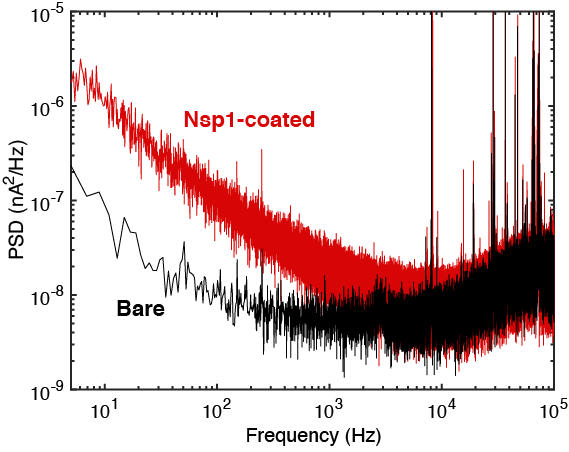
\includegraphics[width=0.7\linewidth]{figures/Figure7.5.png}
	\caption{Current PSD spectra for a bare pore (black) vs a Nsp1-coated pore (red), illustrating the pronounced increase in 1/f noise upon coating the pore with Nsp1.}
	\label{fig:fig7.5}
\end{figure}

\newpage
\subsection{Additional traces of fast Kap95 translocations}

\begin{figure}[!htbp]
	\centering
	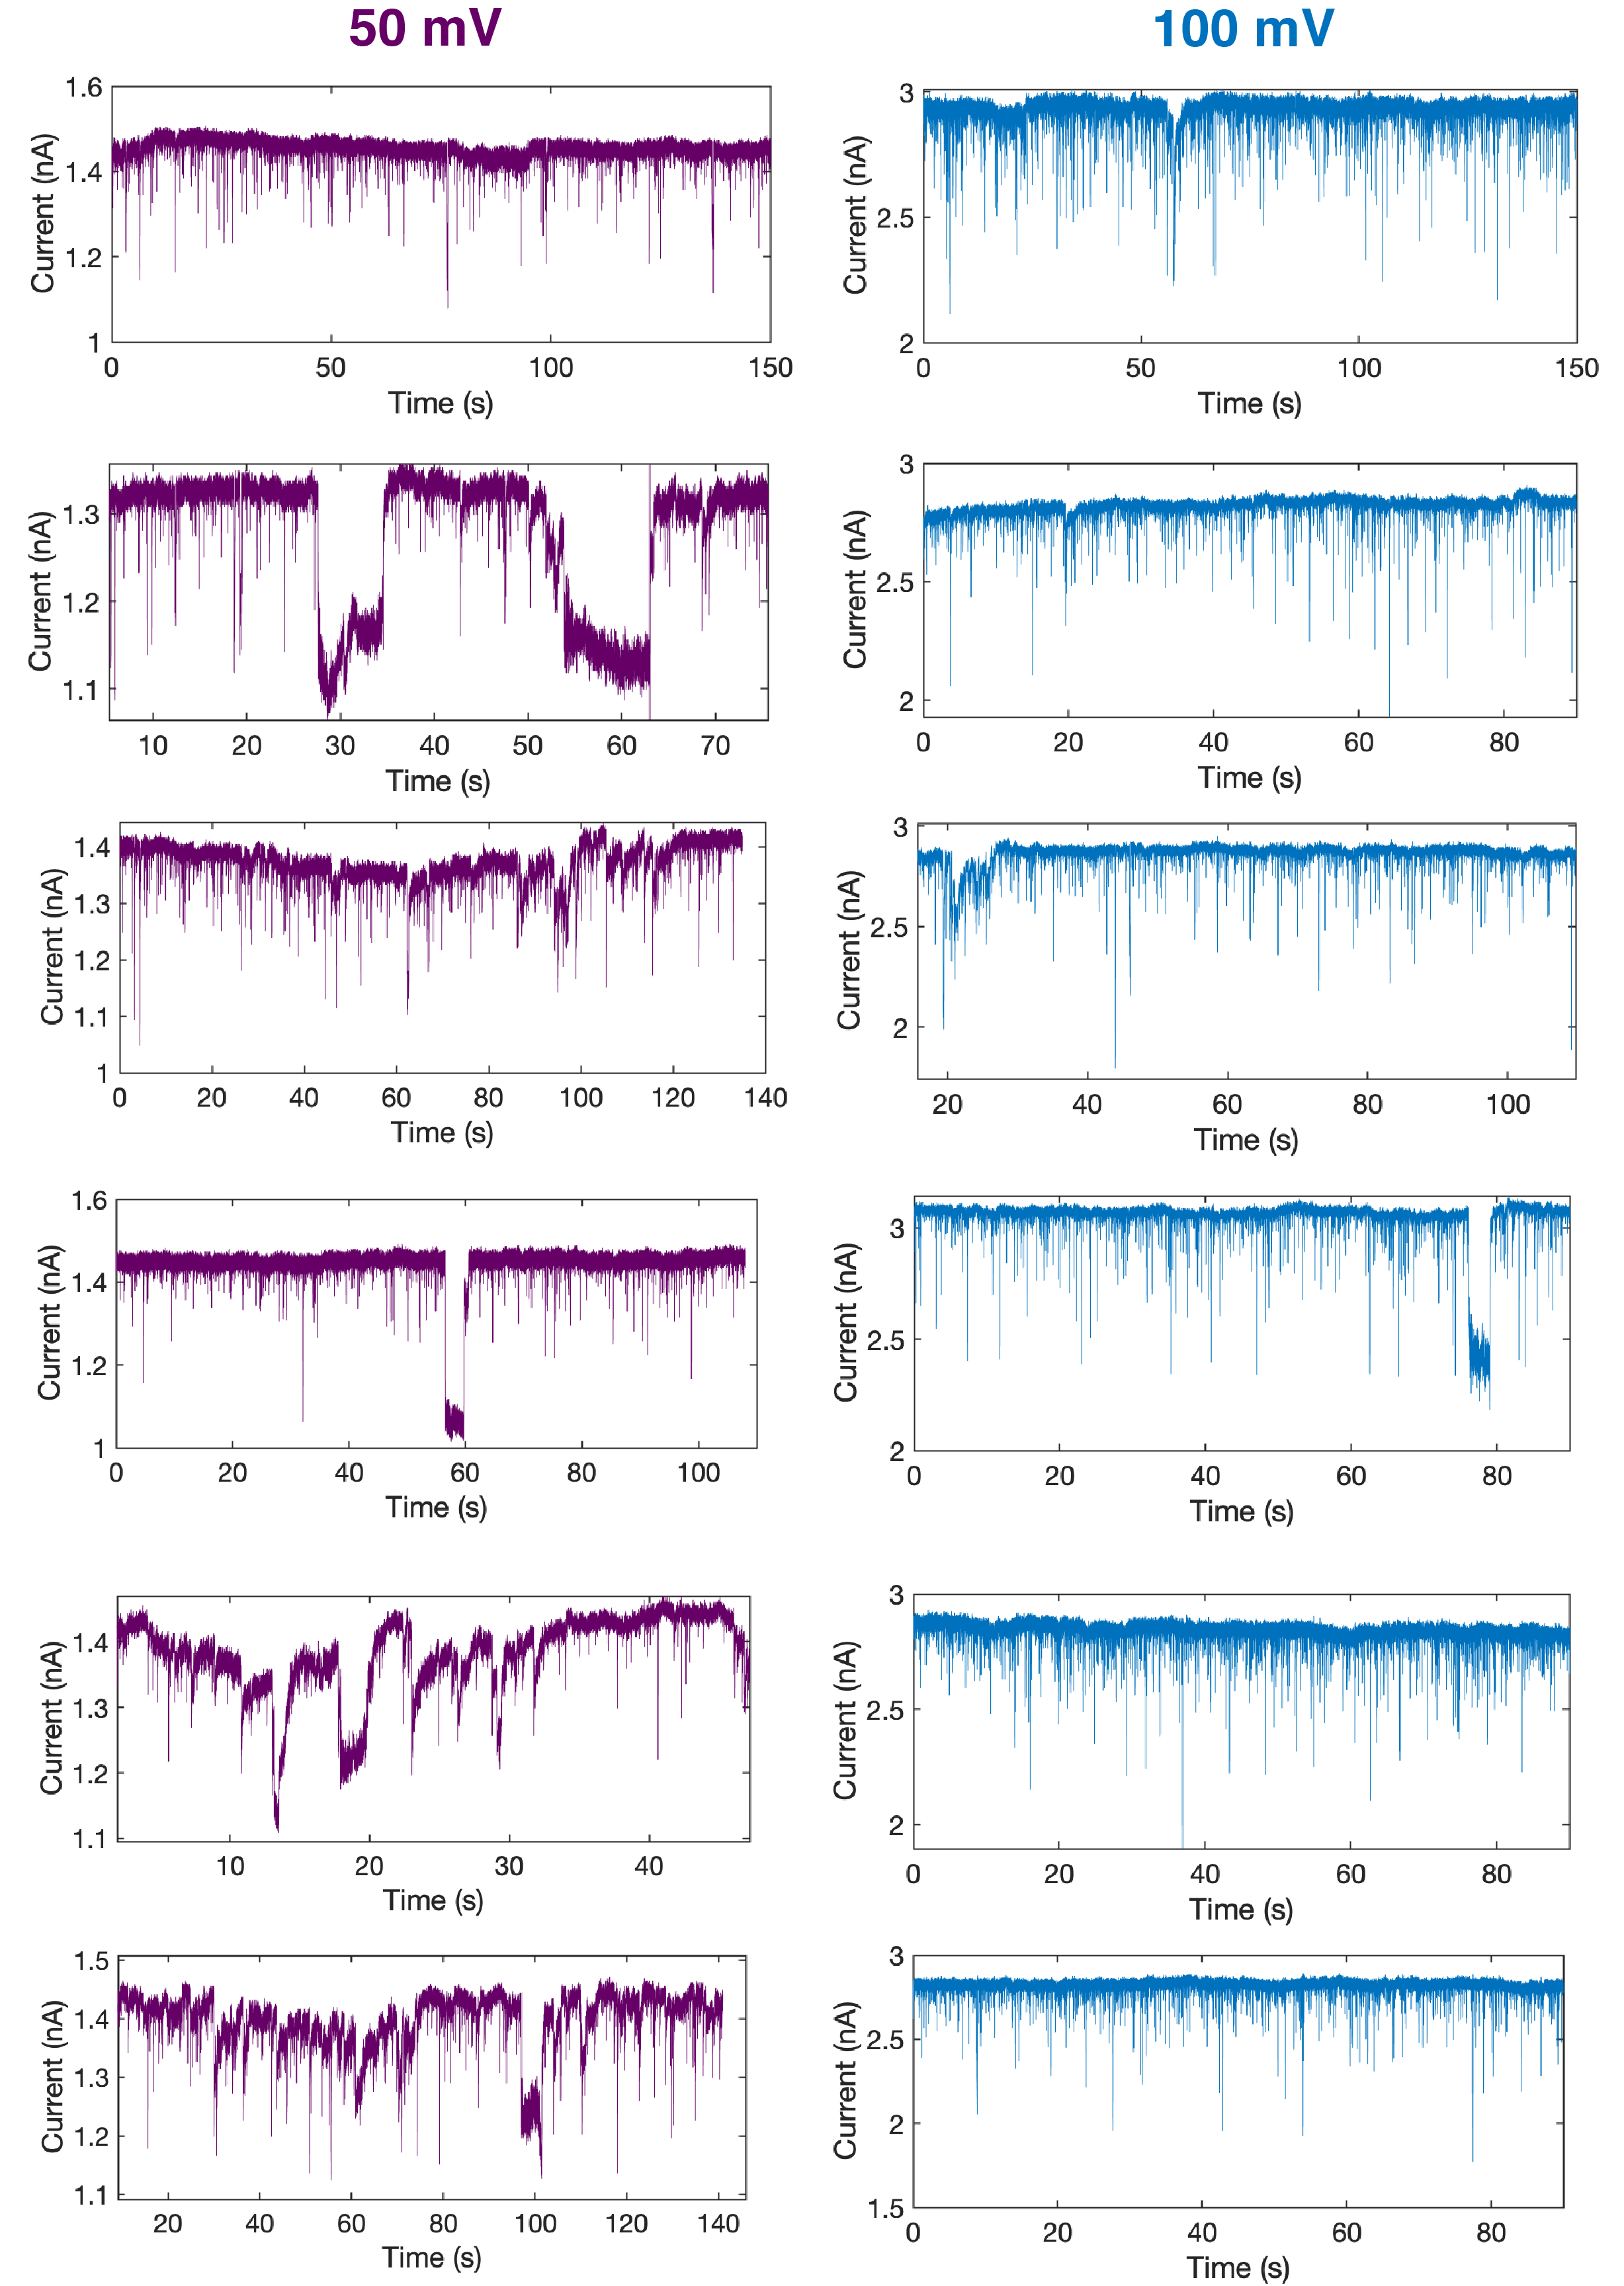
\includegraphics[width=0.9\linewidth]{figures/Figure7.6.png}
	\caption{Additional current traces showing fast Kap95 translocation events through a Nsp1-coated pore under 50mV (left, purple) and 100mV (right, blue).}
	\label{fig:fig7.6}
\end{figure}


\newpage
\renewcommand{\thefigure}{\thechapter.\arabic{figure}}
\renewcommand{\thetable}{\thechapter.\arabic{table}}
\renewcommand{\theequation}{\thechapter.\arabic{equation}}
\references{chapter-7/chapter-7}
